% !Mode:: "TeX:UTF-8:Hard"
\ifx \allfiles \undefined
\documentclass[a4paper,12pt,twoside]{book}
%\usepackage{CJKutf8}
\usepackage[T1]{fontenc}
\usepackage{pifont}
\usepackage{graphicx}
\usepackage{multirow} 
\usepackage{longtable}
\usepackage{capt-of}
\usepackage{color}
\usepackage{amsmath}

\newcommand{\linuxcommand}[1]{\texttt{\textcolor{blue}{\$ #1 \Pisymbol{psy}{191}}}}
\newcommand{\op}[1]{\textcolor{blue}{-#1}}
\newcommand{\hotkey}[1]{\framebox{#1}}
\newenvironment{screen}{\sffamily}{\rmfamily}

% for C/C++ frame box
\usepackage{listings}
\definecolor{mygray}{rgb}{0.9,0.9,0.9}
\lstset{ %
  backgroundcolor=\color{mygray}, basicstyle=\small
}
\lstset{morecomment=[s][\color{red}]{/*-}{*/}}
\newcommand{\Hilight}[1]{\makebox[0pt][l]{\color{yellow}\rule[-3pt]{#1em}{11pt}}}
\newcommand{\HilightLine}[2][yellow]{\makebox[0pt][l]{\color{#1}\rule[-4pt]{#2em}{13.9pt}}}

\newenvironment{answer}{\ttfamily}{\par}

\newcommand{\specialcell}[2][c]{%
  \begin{tabular}[#1]{@{}c@{}}#2\end{tabular}}

\begin{document}
%\begin{CJK*}{UTF8}{song}
\title{Design pattern }
\author{yan zhao}
\date{}\maketitle

\else
\chapter{Design pattern } 
\fi

\section{Basic knowledge}
\begin{itemize}
\item Basic relationships: Inheritance, Dependency, Association, Composition, Aggregation.  \\
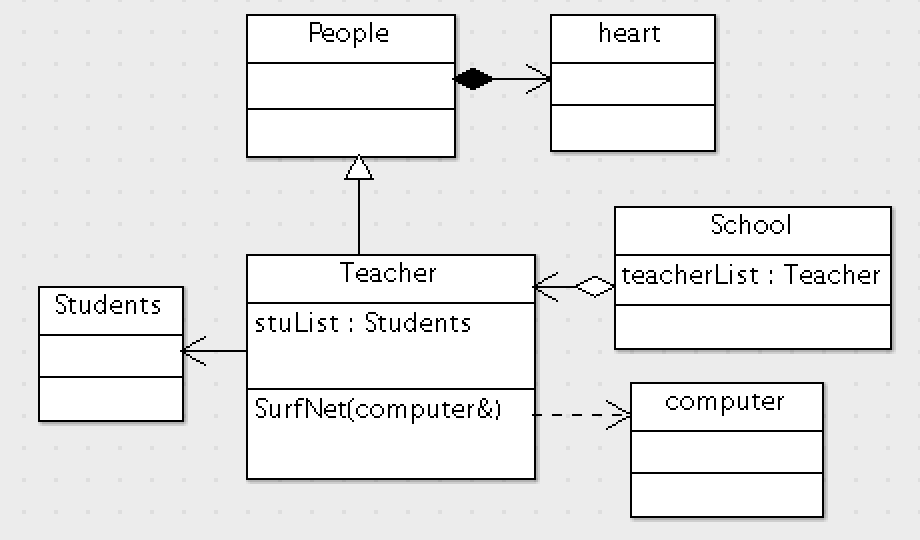
\includegraphics[scale=0.8]{pics/fig.png}

\item Composition is one part of another class, it has \textbf{the same life time} and \textbf{exclusive ownership} such as People and Heart class.

\item Aggregation is a specialized form of Association \textbf{where all objects have their own life time,} and has\textbf{ownership} and one class can't belongs to another class simultaneously. Such as Teacher and School. 

\item Association is a relationship where all objects have \textbf{their own life time} and there is \textbf{no ownership}. Let's take an example of Teacher and Student. Both can create and delete independently.

\item Dependency is weaker relationship. And Class just use another class as method parameter or method return. \textbf{No member in another Class. }  Such as Teacher and Computer. In GOF,  It use dotted line to represent A class create B class. 

\item Basic Ideas:
\begin{enumerate}
\item \textbf{Don't overdesign, Don't use design pattern just because it is here.} Just know some basic design pattern, and follow your real problem, make design fit you problem first, If something changes in the future, you can refactory it later. 

\item Main question in design is: How many classes do you need? Interface of each classes? relationship of Classes(is-a, has-a, and association. ) 

\item When you have all these classes from your practical problem(application), then you need to think three questions. 1) If it's high cohension 2) if it's loose coupling  3) if there is future change. 

\item Then you should use design pattern to design your class again. 

\item Inheritance has three level knowledges.  
\begin{enumerate}
\item The basic knowledge, manager is a person, apple is a fruit, and bla bla bla. 
\item Reused code, pure virtual, virtual, and non virtual, Such as introduced in inheritance section. 
\item \textbf{Isolate change between Client and Implement}. That is the highest level in design pattern. 
\end{enumerate}

\end{enumerate}
\end{itemize}


\section{Basic Principle}
\begin{itemize}

\item Basic principles: 
\begin{enumerate}
\item SRP(Single Responsibility Principle) \textbf{make class interface are complete and minimal.}  That is difficult in practical programming. such as "The zen of Design patterns", A phone class should be derived from IConnetionManager and IDataTransfer. That is an extremely example, but explain some idea of how to keep interface minimal. (In my view, functions should be less than 20. )

\item \textbf{Interface Segregation Principle}. 
\begin{enumerate}
\item Difference between Single Responsibility Principle. SRP consider from inside of a class. Interface Segregation Principle consider from the user of a class. 

\item A simple example is "Interface Segregation Principle" which I have add to my evernote.  If there is robot class, You can't inherit it from IWorker, because robot don't need eat, Maybe you can put an empty function here. but It's not good design. 
\begin{lstlisting}[frame=single, language=c++]
IWorker{
work();
eat()
}
\end{lstlisting}
\end{enumerate}


\item LSP( Liskov Substitution Principle) \textbf{Functions That use pointers or references to base classes must be able to use objects of derived classes without knowing it. }
\begin{enumerate}
\item Subclass must implement all baseclass method.  1) You have to implement pure virtual function.  2) you may or maynot override virtual function.  3) you can't override any non-virtual function. 
\end{enumerate}

\item \textbf{Law of Demeter}
\begin{enumerate}
 \item Basically, class interface should be only include functions. and avoid data members in the public interface.
 \item  \textbf{Only talk with friends Only member. Only input or return parameter in class method are friend.}
 \item An example
 \begin{lstlisting}[frame=single, language=c++]
void method( Teacher & t){
Student s1; // here s1 isn't friend of method. 
t.call(s1);  // should move to Teacher class. 
}
\end{lstlisting}

\end{enumerate}

\item \textbf{Program to an interface, not an implementation. There are another same two principles. They share the same idea behind. }
\begin{enumerate}
\item DIP (Dependence Inversion Principle) High level modules should not depend upon low level modules. Both should depend upon abstraction. 
\item Open close principle (open for extension but closed for modifications.) Allow the adding of new functionality as new classes or inherate current classes, keeping as much as possible existing code unchanged.

\item Subclass extend it's functionality by reusing functionality in parent classes is just inheritance half story, and frankly speaking, not prefer one. \textbf{Favor object composition over object inheritance}

\item Inheritance can make clients remain unaware of specific type of class or obj behind the abstract interface. Then put all change behind the abstract interface. 

\item In C++, you need to declare base class pointer( or reference) and specify a particular implementation obj when you need to change. 

\item How to understand interface? Client<->Interface<->Implement. through Interface, you keep all the change happen implement side, not affect Client at all. 

\end{enumerate}

\item When you want to reuse some codes. \textbf{Favor object composition over class inheritance. }
\end{enumerate}

\end{itemize}

\subsection{High cohension}
\begin{itemize}
\item Data should be private;
\item Small class interface
\item Single Responsibility principle
\end{itemize}

\subsection{Loose coupling}
\begin{itemize}
\item  Build a middle class to decrease coupling.  \\
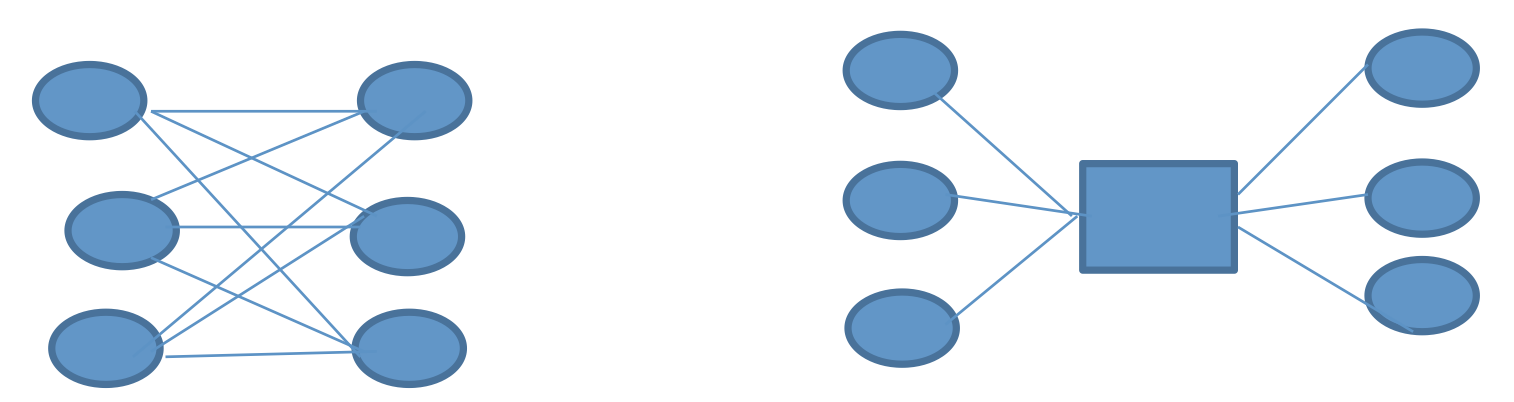
\includegraphics[scale=0.45]{pics/middle.png}
\end{itemize}

\section{Design pattern}
\subsection{Introduction}
\begin{itemize}

\item Don't understand Design pattern by language. Such as factory method and template method, They share the same language structure( class inheritance and structure). But their context is different. 

\item Easy pattern: singleton, Facade, adapter, mediator,  observe, Prototype, strategy, factory method, template mehod, command, proxy, memento. 

\item Three use recursive: composite, decorator, chain of responsibility and Interpreter. 

\item Bridge , abstractor factory and visitor have same points, they all  have parallel two inheritance system, there is a relationship between two systems. 

\item Template method and Factory method are both \textbf{pull up common and push down change}. Template pull up common algorithm steps and Create templateMethod(). And Factory method pull up common produced procession and Create factoryMethod.

\item Sometimes, You want to pull up common. But there is NO concrete conception(A noun) waiting here, then you can abstract a conception, and make an abstract class as base class. 
\begin{enumerate}
\item Button and applicaition should not have baseclass, but they both support requestHandle(), So you create Handler class.
\item Textview and decorator should not have base class, but after decoration, textview is still textview.  So I create VisualComponent Base class.
\item In Mediator pattern. Listbox and EntryField have now common baseclass, So create Colleague baseclass. 
\item  Proxy is also follow this idea.
\end{enumerate}
   
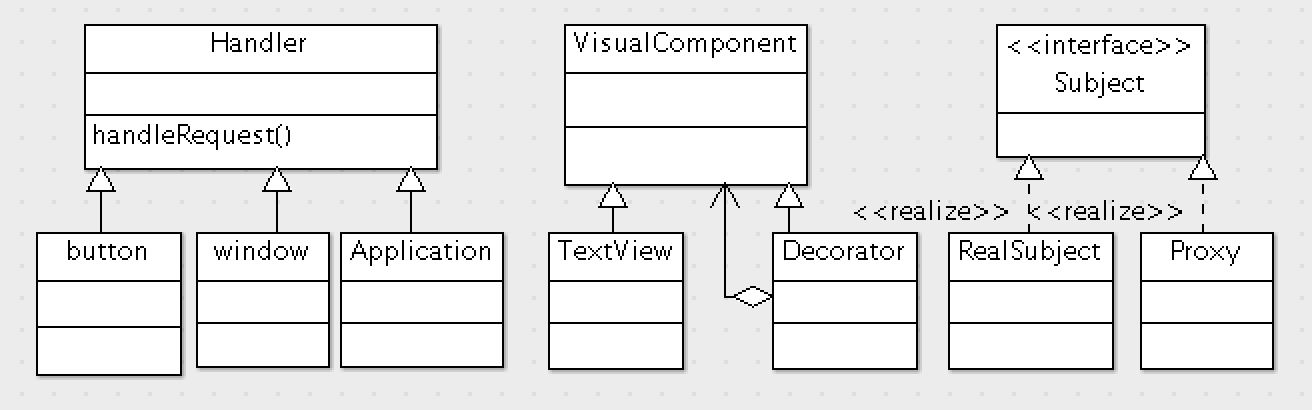
\includegraphics[scale=0.6]{pics/common.png}

\item Program to interface. But where are interfaces?  
\begin{enumerate}
\item You can pull up to create baseclass interface: such as \textbf{component, chain of responsible, decorator and proxy.}  
\item You can create a medium class(interface) . such as \textbf{command} between invoker and Receiver, \textbf{Memento} between Originator and caretaker.  \textbf{adapter} between Target and Adaptee. \textbf{Mediator} between Colleague and ConcreteMediator. 
\item \textbf{Iterator} between container and algorithms. \textbf{builder} between Director and product.  
\end{enumerate}


\end{itemize}

\subsection{Creational patterns}
\subsubsection{Singleton}
\begin{itemize}
\item Singleton: A class of which only a single instance can exist. Ensure a class only has one instance, and provide a global point of access to it.

\item Don't need fig, just remember implementation.  \textbf{One class, two static, three access levels(private, protect, public) }  
\begin{lstlisting}[frame=single, language=c++]
class Singleton{
private:
   static Singleton * m_instance;
protect
   Singleton();
public:
  static getInstance(); 
}

Singleton* Singleton::m_instance = nullptr;
Singleton::getInstance(){
  if(m_instance == nullptr)
     m_instance = new Singleton();
   return m_instance;
}
\end{lstlisting}


\end{itemize}

\subsubsection{Prototype}
\begin{itemize}
\item A fully initialized instance to be copied or cloned. Specify the kinds of objects to create using a prototypical instance, and create new objects by copying this prototype.

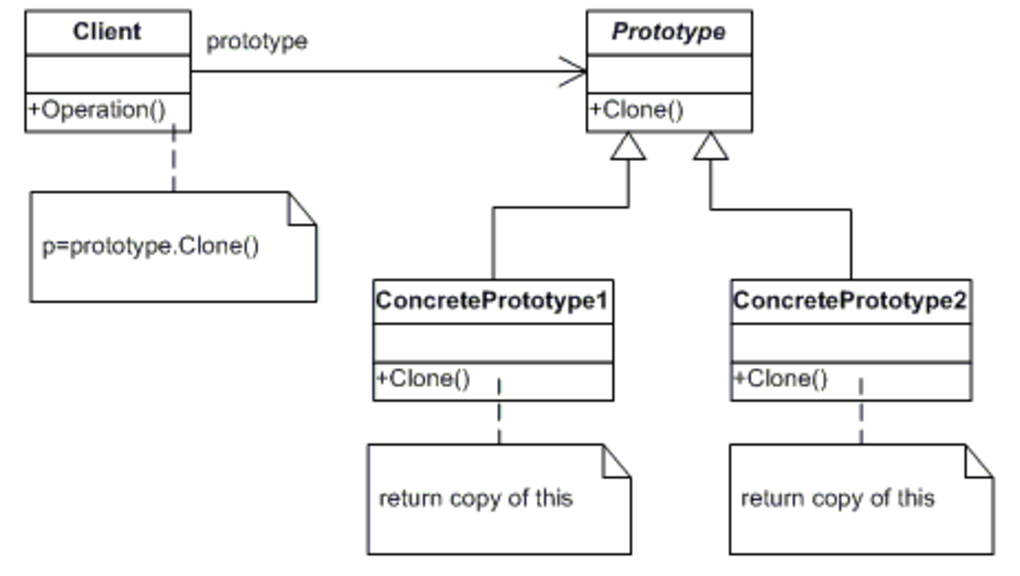
\includegraphics[scale=0.65]{pics/prototype.png}

\item There are two advantages of clone. 1)It can reduces complex and growing class contruction time.  2)Sometimes, you don't know what kind of object should be created, For example, passing an abstract product obj pionter , at this time, you don't know what kind of child class it pointed.  You can use RTTI, But a better method is to use clone() directly. 
\begin{lstlisting}[frame=single, language=c++]
Create(absproduct * absp){
// use RTTI on absp; not good
absp->clone(); // this a good.
}
\end{lstlisting}

\item In C\#, base class object include clone() method.  it just use binary stream way to clone a object. In Java, you can extend IClone interface. clone is so important, it become a "build-in" feature in Java or C\# language. 

\item In C++, you can just add clone method in your class if you want to it support clone. You don't need to create a baseClass with virtual clone(), then inheriate you present class from it. 

\item But in a music note example, There are HalfNote and WholeNote classes, and dragMusicNote() need to support them all. At this time, you need to create a prototype baseClass, and make you HalfNote and WholeNote derived from it. Just like previous figure show. 

\begin{lstlisting}[frame=single, language=c++]
dragMusicNote(Note* p){
Note* pNew = p->clone();
pNew->draw();
}
\end{lstlisting}

\item MusicNote give us a good hint. \textbf{Inheritance is a 1) is-a relationship, 2) You also can use it when it subclass and baseclass both support some actions. such as clone(). } 

\item Inside clone(), you can use new return a pointer, or use(*this) return a value.  

\end{itemize}

\subsubsection{Factory method}
\begin{itemize}
\item Factory Method: Creates an instance of several derived classes. Define an interface for creating an object, but let subclasses decide which class to instantiate. Factory Method lets a class defer instantiation to subclasses.

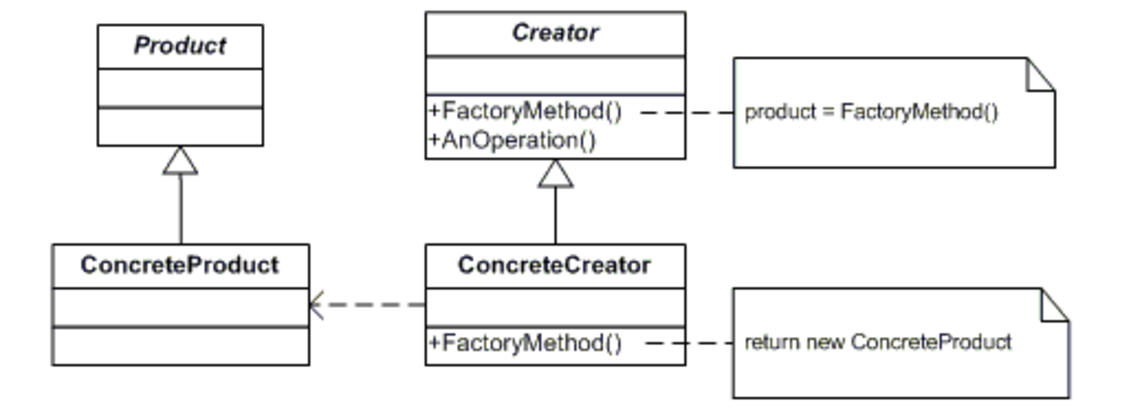
\includegraphics[scale=0.66]{pics/ft.png}

\item \textbf{In fact, this pattern is jut method, and this method produce a object, so call factory method.}
\item In previous, Creator is not good name for this class name, A better name is Applicaiton. Because this Application just need this Product in AnOperation(). Application's main goal isn't producing a object. You need to know this. 

\item Application(Creator in previous fig) want to use produce, But only subclass know what kind of ConcreteProduct will be produced. Ok, The main common points is a product will be produced, So I pull up this common point and put it in base class, call it virtual FactoryMethod(). Then push down all change to subclass. It's good idea of\textbf{pull up common and push down change}

\end{itemize}

\subsubsection{Abstract Factory}
\begin{itemize}
\item Creates an instance of several families of classes. Provide an interface for creating families of related or dependent objects without specifying their concrete classes.

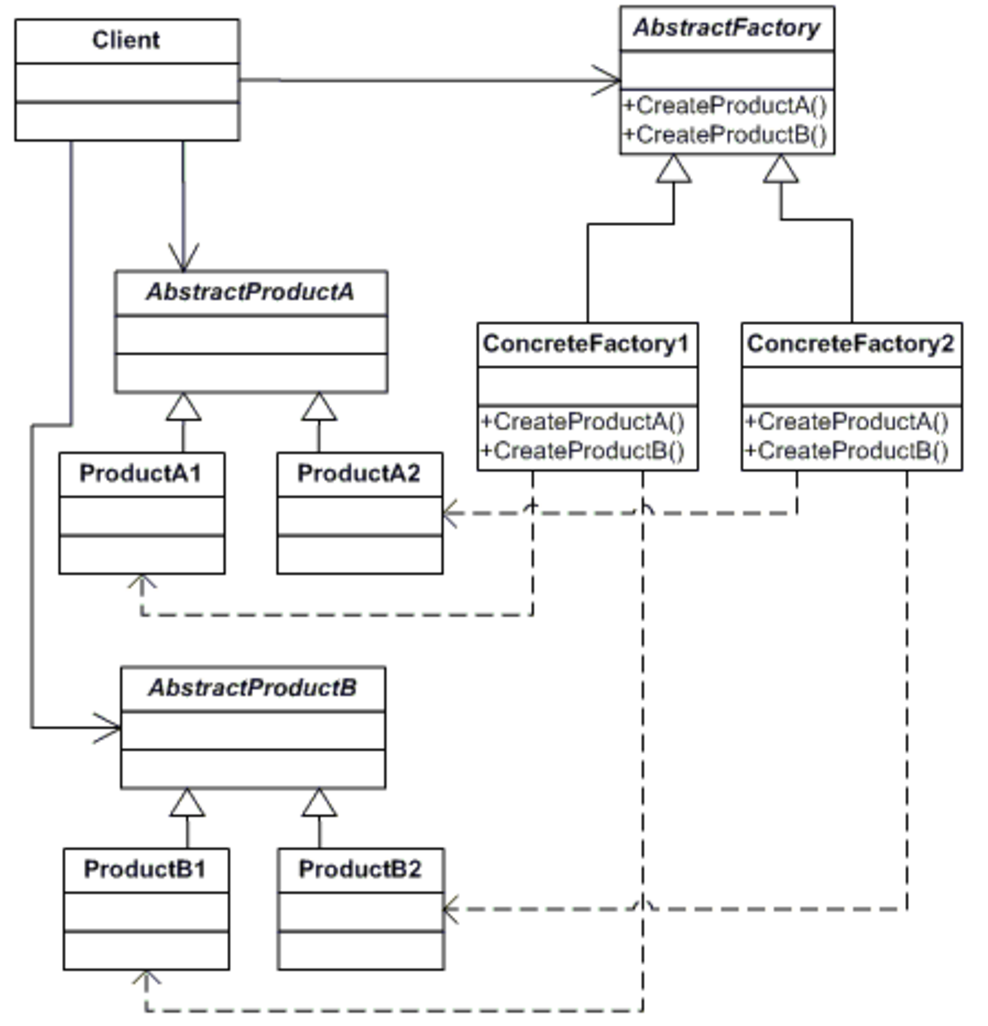
\includegraphics[scale=0.75]{pics/abstractFactory.png}

\item Client just use abstractFactory and abstractProduce two interfaces. When you input different concrete abstractFactory, products are changed accordingly. 

\end{itemize}

\subsubsection{Builder}
\begin{itemize}
\item Separates object construction from its representation. Separate the construction of a complex object from its representation so that the same construction processes can create different representations.

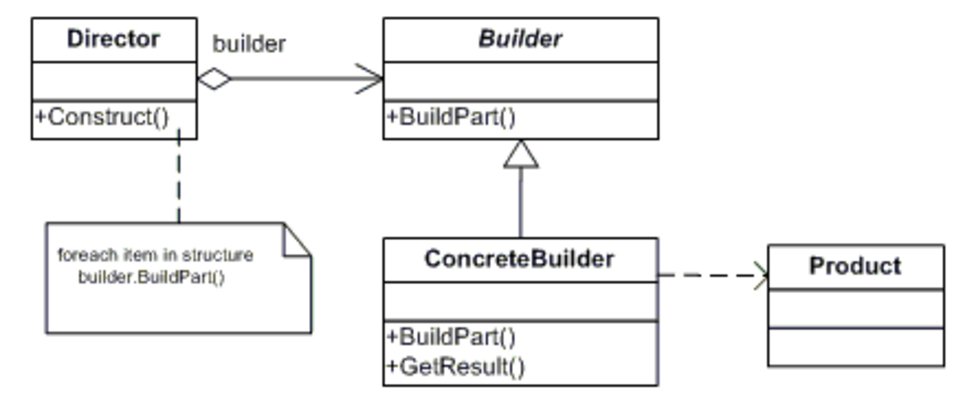
\includegraphics[scale=0.75]{pics/builder.png}

\item Builder focuses on constructing a complex object step by step. Abstract Factory emphasizes a family of product objects(eighter simple or complex). Builder returns the product as a final step, but as far as the abstract Factory is concerned, the rpdocuct gets returned immediately. 

\item Composite most produced by builder. 
\item builder is included by a director. 

\item 
\end{itemize}

\subsubsection{Creational summary} 
\begin{itemize}
\item Often, design start out using Factory method( less complicated, more customizable, subclasses proliferate) and evolve toward Abstract Factory, Prototype, or Builder( more flexible, more complex) as the designer discovers where more flexibbility is needed. 
\item Sometimes creational patterns are complementary: Builder can use one of the other patterns to implement with components get build. 
\end{itemize}


\subsection{Structurtal patterns}
\subsubsection{Adapter}
\begin{itemize}
\item Adapter: Match interfaces of different classes.Convert the interface of a class into another interface clients expect. Adapter lets classes work together that couldn’t otherwise because of incompatible interfaces.

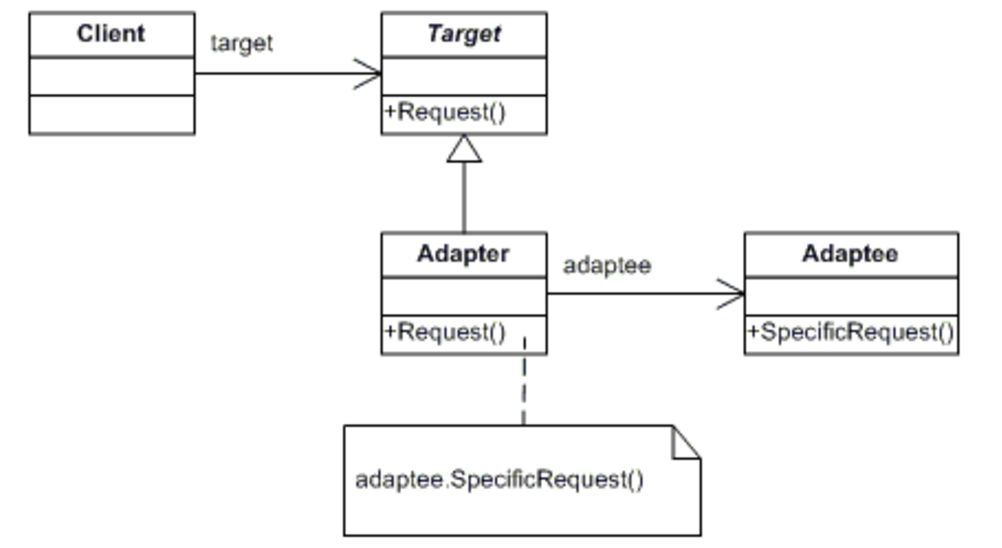
\includegraphics[scale=0.75]{pics/adapter.png}

\item Know adaptee of adapter.  It can be implemented by private inheritance adaptee or contian an adaptee object. 

\item adapter reuse an interface, facade define a new interface. 

\end{itemize}

\subsubsection{Bridge }
\begin{itemize}
\item Bridge: Separates an object’s interface from its implementation. Decouple an abstraction from its implementation so that the two can vary independently.

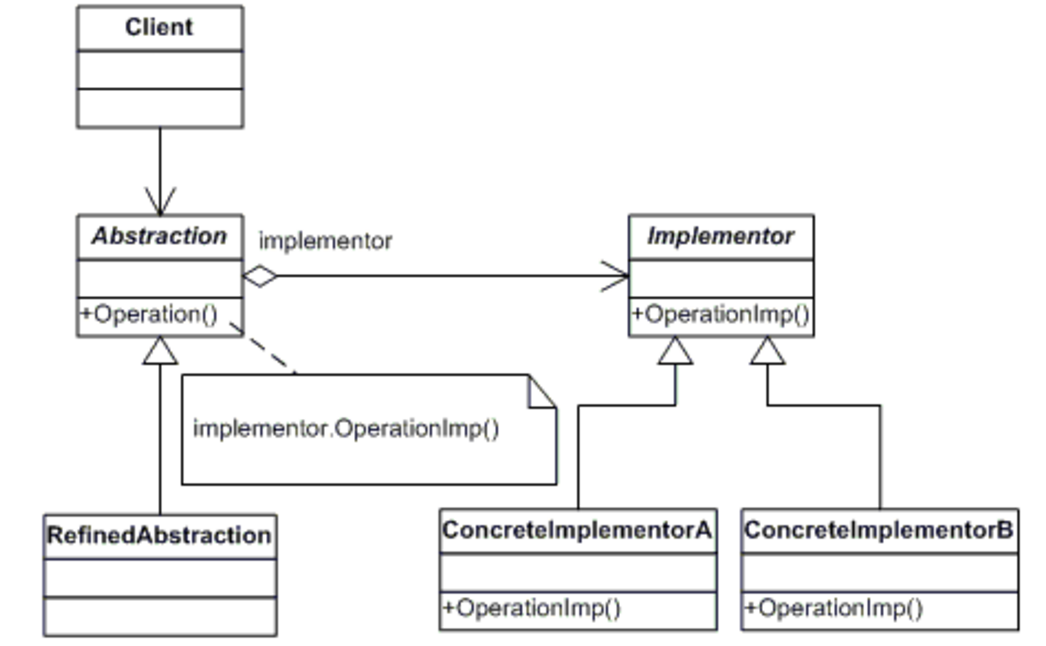
\includegraphics[scale=0.69]{pics/bridge.png}

\item Gof narrow bridge to abstract and implementation. It's proper for the example in Gof Example. But we should think it wider. If we have A and B, they both flexible and easy to extend, at the same time, there is relationship between A and B, such as implementation(Bridge) produce(abstract Factor), Visit(Visitor), then we should consider use it. 
\end{itemize}

\subsubsection{Composite}
\begin{itemize}
\item Composite: A tree structure of simple and composite objects. Compose objects into tree structures to represent part-whole hierarchies. Composite lets clients treat individual objects and compositions of objects uniformly.

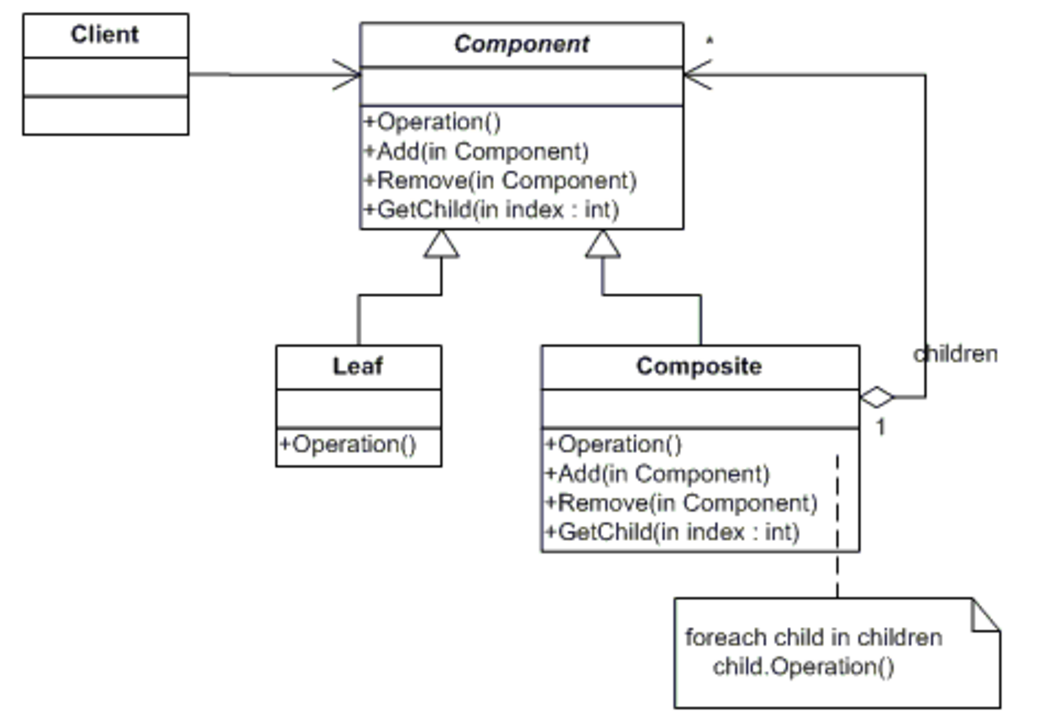
\includegraphics[scale=0.69]{pics/composite.png}

\item It can be use as recursive Tree structure. Such as file tree. A folder is composite, and a file is component, and a folder can be a component of another composite. 

\item Client just communicate with abstract component, invoke it's operation function. 

\item A leaf will not include any component. 

\item Composite has a children component list. It has add(), remove() and getChildren() three functions. 

\item You can add component \&parent, then It will point to parent 
\end{itemize}

\subsubsection{Decorator}
\begin{itemize}
\item Decorator: Add responsibilities to objects dynamically.  Attach additional responsibilities to an object dynamically. Decorators provide a flexible alternative to subclassing for extending functionality.
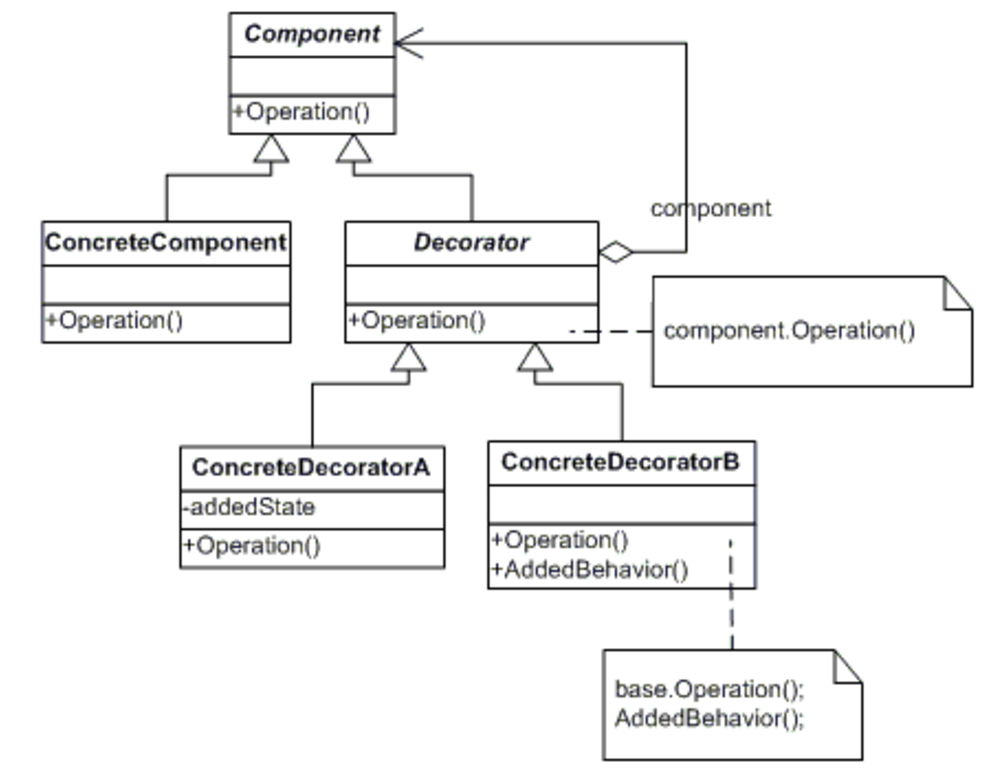
\includegraphics[scale=0.75]{pics/decorator.png}

\item Nearly same with composite. you can think it as "only one component composite".  But it is not aggregation of object, but add a layer of decoration. 

\item decorate avoid static implement all permutation. composite make all component can be deal with in the same manner. 

\item In Gof example, If we don't use decorator. We need to inherit from textview and produce scrolltextview and bordertextview. At this time, if we need scroll and border together, we also need to define scroolbordertextview class. It's very bad design. 1) it will produce too many classes and 2) you can't change it dynamically. 


\end{itemize}

\subsubsection{Facade}
\begin{itemize}
\item Facade: A single class that represents an entire subsystem. Provide a unified interface to a set of interfaces in a system. Facade defines a higher-level interface that makes the subsystem easier to use.

\end{itemize}

\subsubsection{Proxy}
\begin{itemize}
\item Proxy: An object representing another object. Provide a surrogate or placeholder for another object to control access to it.

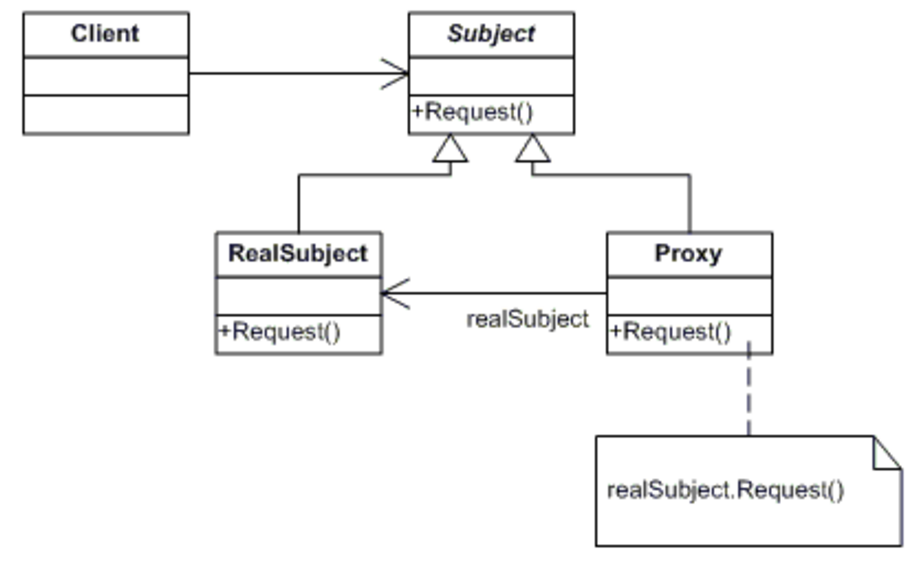
\includegraphics[scale=0.69]{pics/proxy.png}

\end{itemize}

\subsubsection{Flyweight}
\begin{itemize}
\item Flyweight: A fine-grained instance used for efficient sharing. Use sharing to support large numbers of fine-grained objects efficiently. A flyweight is a shared object that can be used in multiple contexts simultaneously. The flyweight acts as an independent object in each context — it's indistinguishable from an instance of the object that's not shared.

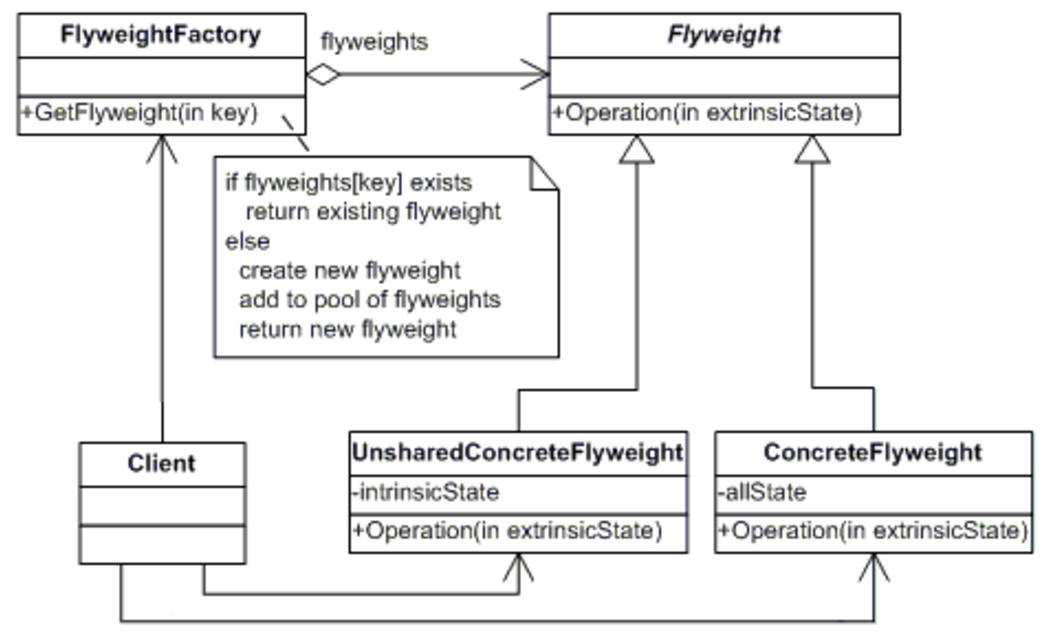
\includegraphics[scale=0.69]{pics/fly.png}

\item Flyweight just keep intrinsic state, and all the extrinsic states are kept outside of object. 

\item An application uses a large number of objects, and most object state can be made extrinsic. 

\end{itemize}


\subsection{Behavioral  patterns}

\subsubsection{Observer}
\begin{itemize}
\item Observer: A way of notifying change to a number of classes. Define a one-to-many dependency between objects so that when one object changes state, all its dependents are notified and updated automatically.

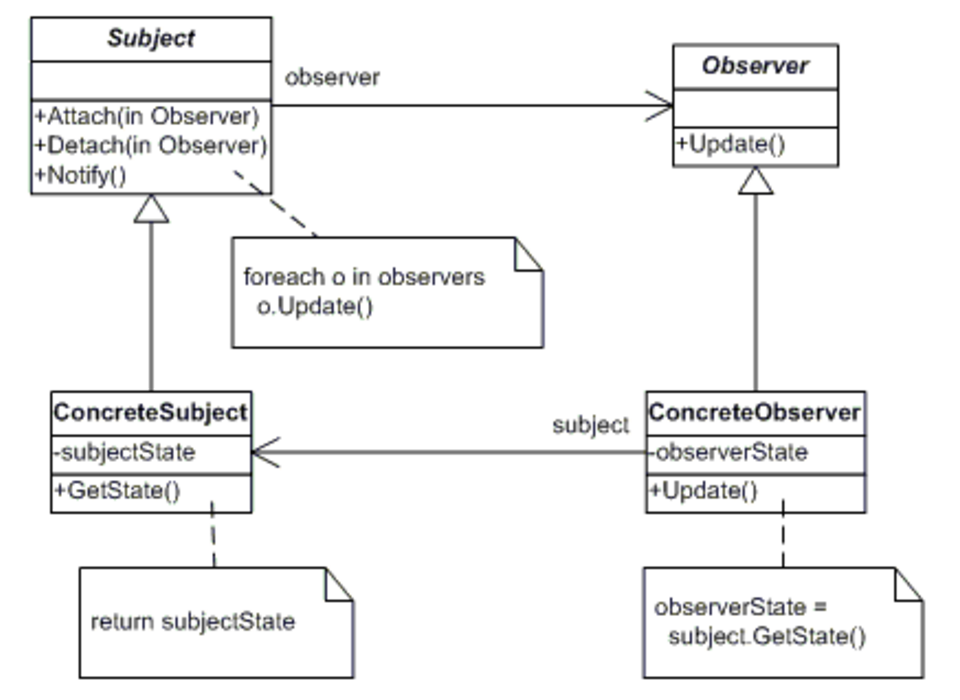
\includegraphics[scale=0.69]{pics/observer.png}

\item One Observer, include update(), One Subject, includes addObserve(), deleteObserve(), notify()

\item Observer chain effect. an Observer is both a Observe and a Subject. 

\item Pass what to update()? It can be big, such as update(Subject *s).  It can be small, such as update(string\& ).  It's a practical problem. 

\end{itemize}

\subsubsection{Mediator}
\begin{itemize}
\item Mediator: Defines simplified communication between classes. Define an object that encapsulates how a set of objects interact. Mediator promotes loose coupling by keeping objects from referring to each other explicitly, and it lets you vary their interaction independently.

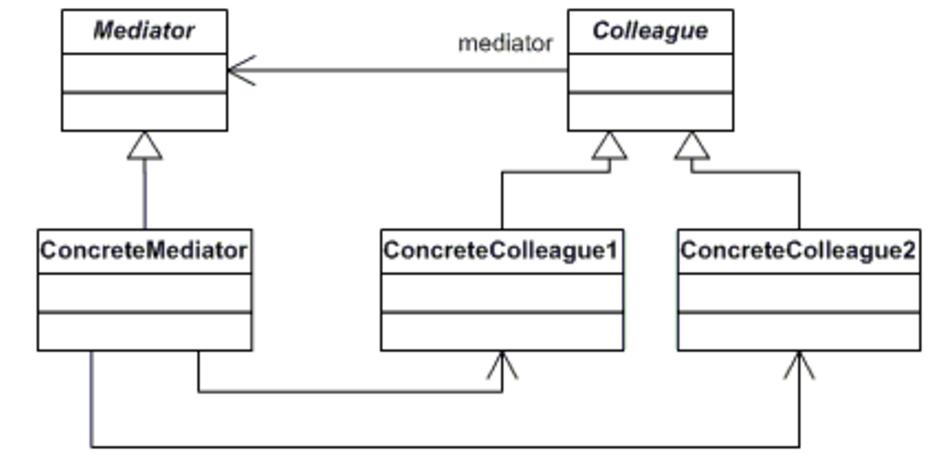
\includegraphics[scale=0.75]{pics/mediator.png}

\item There is similarity between Mediator and Observer.  For Mediator: all colleagues use mediator.colleaguesChange(this) to notify one Mediator.  For observer: one subject use observer.update(this) to notify all observers.

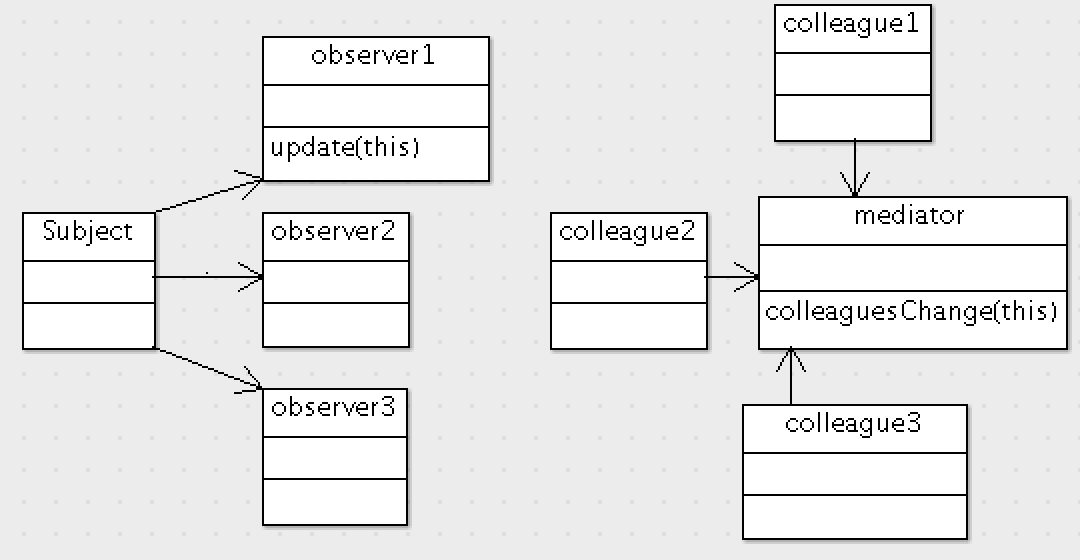
\includegraphics[scale=0.6]{pics/om.png}
\end{itemize}




\subsubsection{State}
\begin{itemize}
\item State: Alter an object's behavior when its state changes. Allow an object to alter its behavior when its internal state changes. The object will appear to change its class.

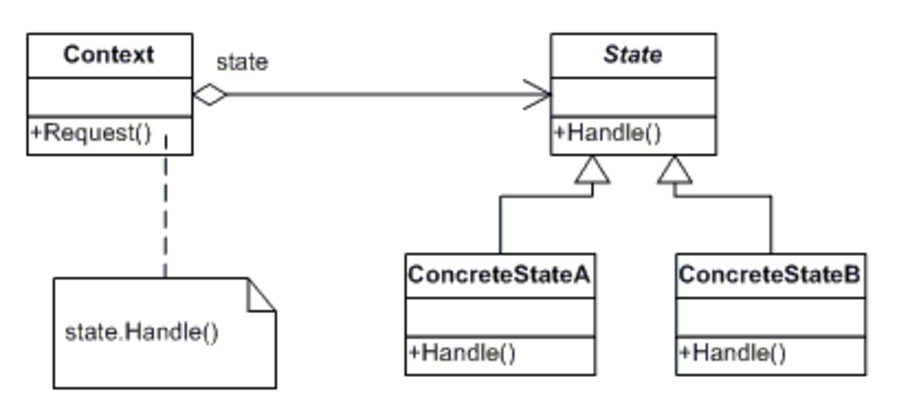
\includegraphics[scale=0.8]{pics/state.png}

\item In side of context:
\begin{enumerate}
\item keep a reference of current state.
\item delegate all action by current state. 
\item keep static const state as how many states you have
\end{enumerate}

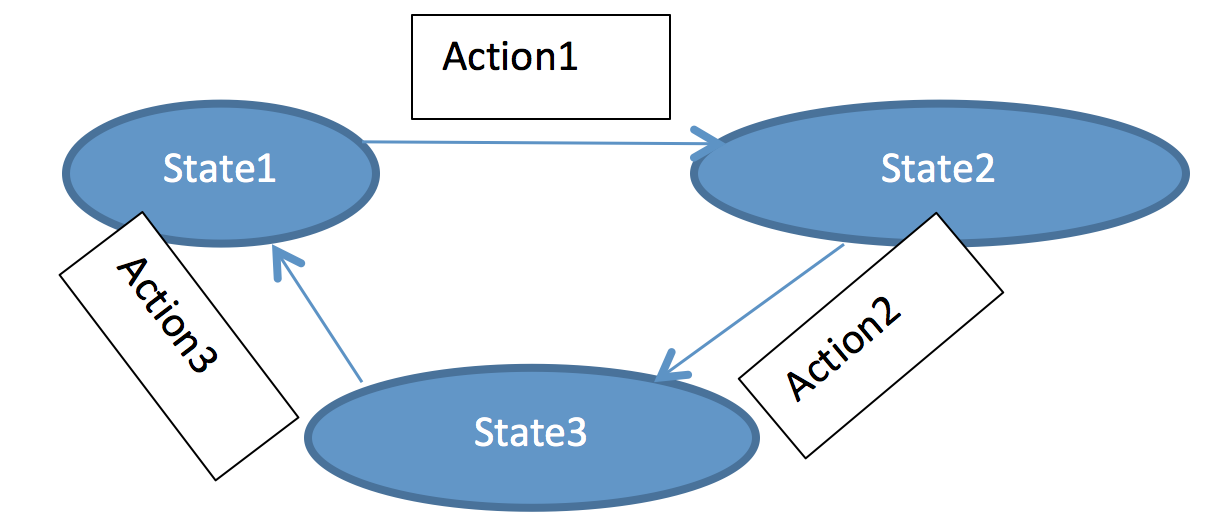
\includegraphics[scale=0.5]{pics/statechange.png}

\item In side of concreteState:

\begin{enumerate}
\item manage of current state
\item transmission of states.
\item In all concreteState, you need to define all the actions, even some actions is meanless, just leave it empty. 
\end{enumerate}

\end{itemize}

\subsubsection{Chain of responsibility}
\begin{itemize}
\item Chain of Resp. : A way of passing a request between a chain of objects. Avoid coupling the sender of a request to its receiver by giving more than one object a  chance to handle the request. Chain the receiving objects and pass the request along the chain until an object handles it.

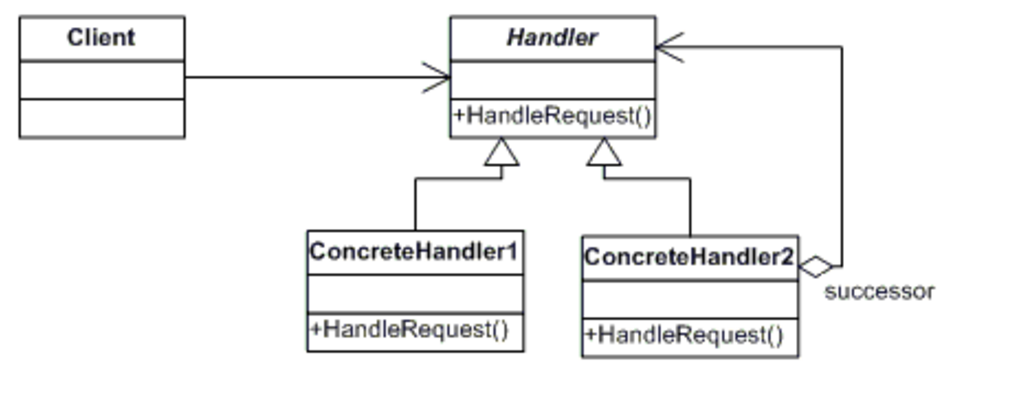
\includegraphics[scale=0.8]{pics/chain.png}

\item In each concrete handler, You need to 1) judge if you should handle(), 2) set next successor. 

\item Just like composite, but it only include one successor. 

\item How to judge if I handle a request or pass it to the success, you can hard code it or make a request class. 

\item 
\end{itemize}


\subsubsection{Command}
\begin{itemize}
\item Command: Encapsulate a command request as an object. Encapsulate a request as an object, thereby letting you parameterize clients with different requests, queue or log requests, and support undoable operations.
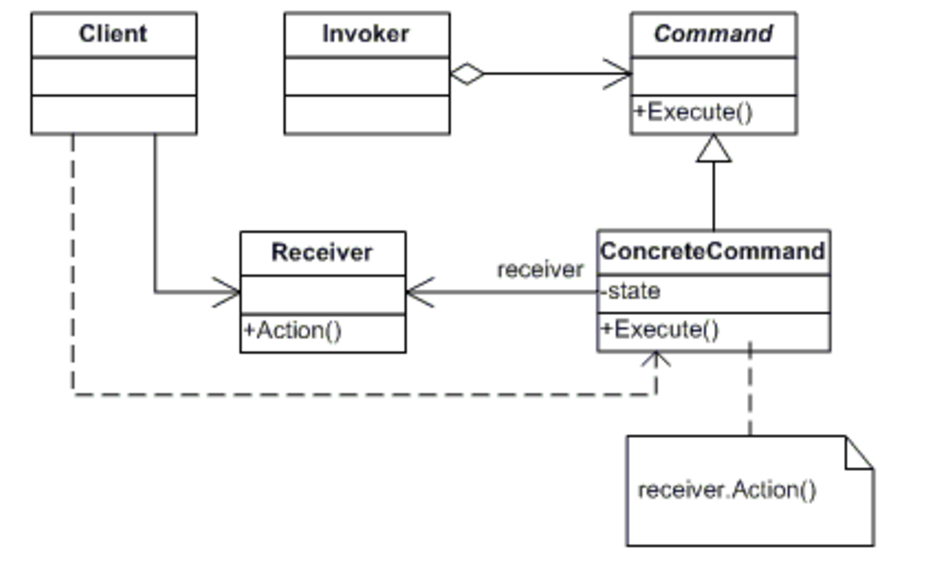
\includegraphics[scale=0.75]{pics/command.png}

\item decoupling between invoker and carrier of a command. 

\item single command is easy. Using command, you can 1) log of command, 2) undo a command 3) Transaction of command. They are more valuable. 

\item Execute() is only method in command class. 
\end{itemize}

\subsubsection{Memento}
\begin{itemize}
\item Memento: Capture and restore an object's internal state. Without violating encapsulation, capture and externalize an object’s internal state so that the object can be restored to this state later.

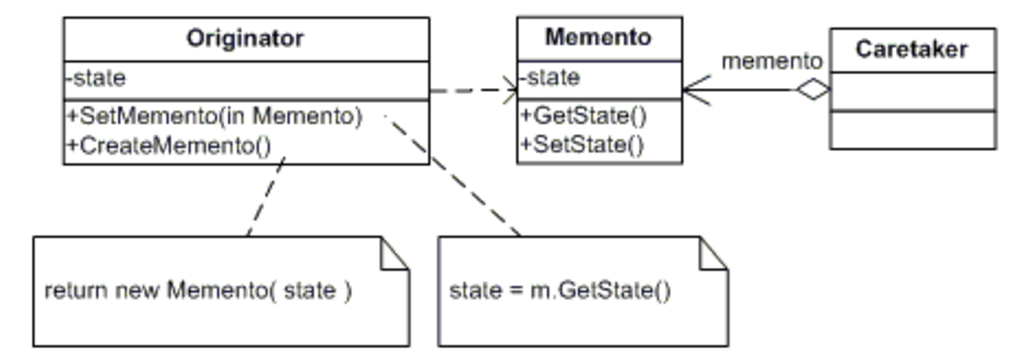
\includegraphics[scale=0.65]{pics/memento.png}

\item Don't damage encapsulation of Originator,  catch a snapshoot inside state (memento), save it in the caretaker, Then call SetMemento inside of originator to restore it. 
\end{itemize}

\subsubsection{Iterator}
\begin{itemize}
\item Iterator: Sequentially access the elements of a collection. Provide a way to access the elements of an aggregate object sequentially without exposing its underlying representation.

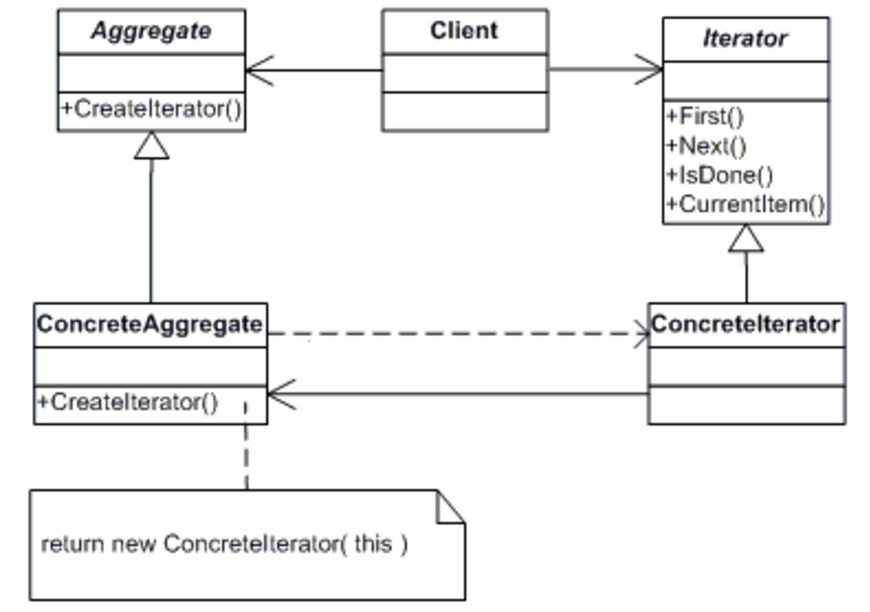
\includegraphics[scale=0.8]{pics/iterator.png}


\end{itemize}

\subsubsection{Visitor}
\begin{itemize}
\item Visitor: Defines a new operation to a class without change. Represent an operation to be performed on the elements of an object structure. Visitor lets you define a new operation without changing the classes of the elements on which it operates.

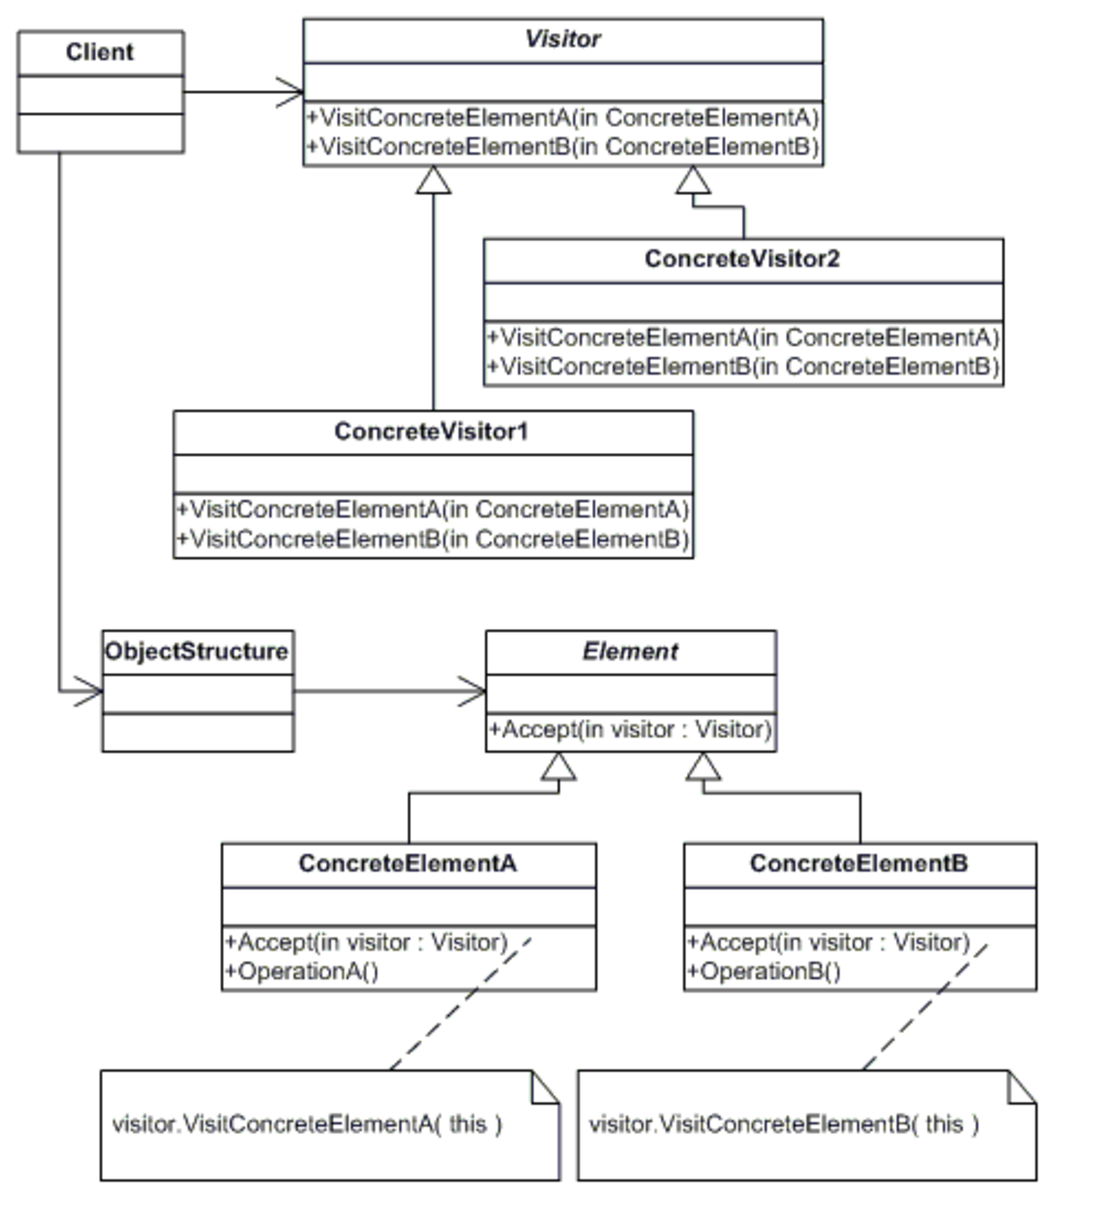
\includegraphics[scale=0.75]{pics/visitor.png}

\item Different with observer, Don't think observe even a bit when you try to understand visitor. They are totally different. 

\begin{enumerate}
\item You have a solid class structure.  I don't add or delete class from this structure. (Structure of company usually is stable)
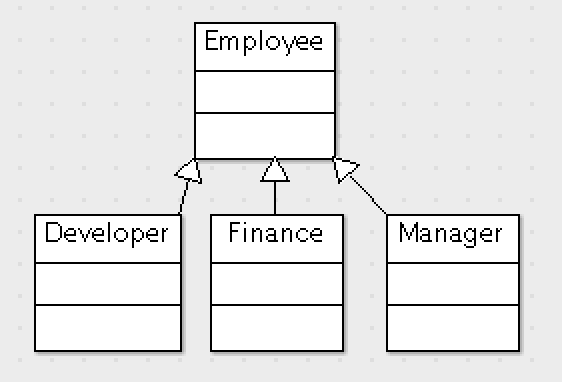
\includegraphics[scale=0.75]{pics/v1.png}

\item You have a container to contain these objs( All empoyees in one company ). and you need to loop these objs to apply an operation. For different kind objs, operation should be a little different. (calculateSalary() operation ,Manager*1.5, and Developer*1.2). A nature way is to define calculateSalary virutal function in base class. 

\item Problem one is We need add another operation, such as audit(), performance(), bodycheck()..... Whenever you add an operation, you need to change all class interface. 

\item Problem two is WE mush put all kinds of operation into one class.  Furthermore, some common parts  have to distribute among different class. 

\item \textbf{class structure solid, but operation flexible. } You can abstract each operation as a concreteVisitor.  \textbf{Add operation is easy, but changing  class in class struture is very difficult. }

\item If container include different type of class, for example, company container include all Employee objs and also include Car objs, This time, visitor pattern is you only option.  


\end{enumerate}

\end{itemize}

\subsubsection{Interpreter}
\begin{itemize}
\item Interpreter: A way to include language elements in a program. Given a language, define a representation for its grammar along with an interpreter that uses the representation to interpret sentences in the language.

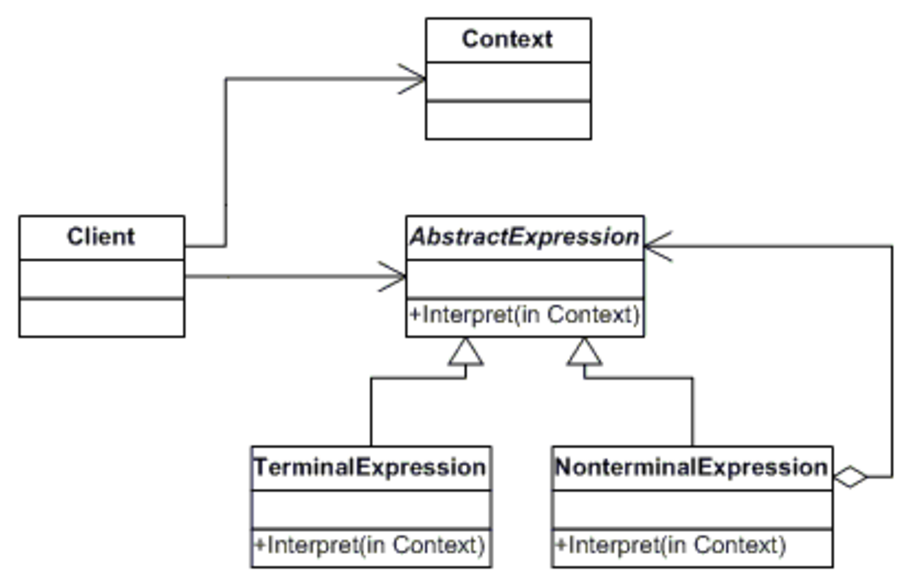
\includegraphics[scale=0.75]{pics/interpreter.png}

\item This pattern doesn't use very often.  It can be thought as a special case of composite pattern.
\begin{enumerate}
\item You need to have a grammar. This is start symbol is Expression. VarExp is leaf. That is a context free grammer
\begin{lstlisting}[frame=single, language=c++]
Expression ::= AddExp | SubExp | VarExp
VarExp ::=1|2|3|4|5
AddExp ::= Expression + Expression
SubExp ::= Expression - Expression
\end{lstlisting}

\item With this grammer, you can design class diagram as below: 

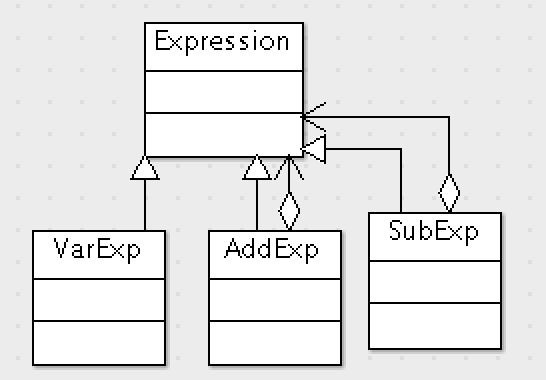
\includegraphics[scale=0.75]{pics/exp.png}

\item For this prammer, You need to parse a sentence defined by this grammar. The last purpose of parsing is to calculate the value of expression. So interprete() should be a calculate function. and interprete will be called recursively. 

\item parse function is not key problem to be solved by Interpreter patten. For regular grammar, you can use FST, for simple arithmetic( this example), You can use stack and scan a terminal in an expression from left to right. 
\item 


\end{enumerate}

\end{itemize}


\subsubsection{Strategy}
\begin{itemize}
\item Strategy: Encapsulates an algorithm inside a class. Define a family of algorithms, encapsulate each one, and make them interchangeable.            Strategy lets the algorithm vary independently from clients that use it.

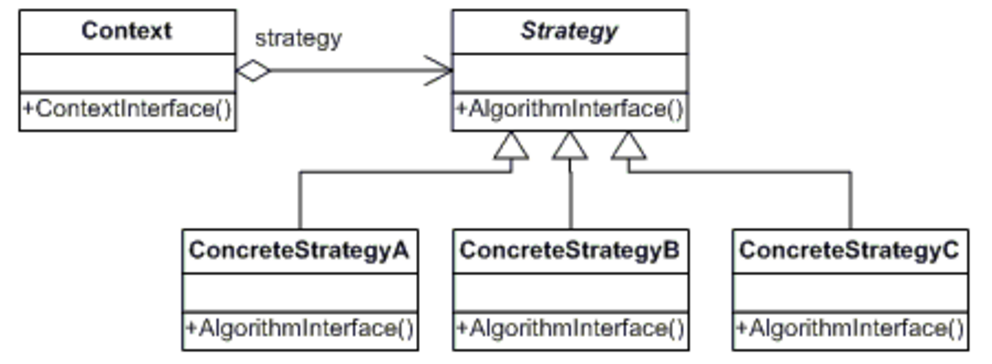
\includegraphics[scale=0.75]{pics/strategy.png}

\end{itemize}

\subsubsection{Template method}
\begin{itemize}
\item Template method: Defer the exact steps of an algorithm to a subclass. Define the skeleton of an algorithm in an operation, deferring some steps to subclasses. Template Method lets subclasses redefine certain steps of an algorithm without changing the algorithm’s structure.

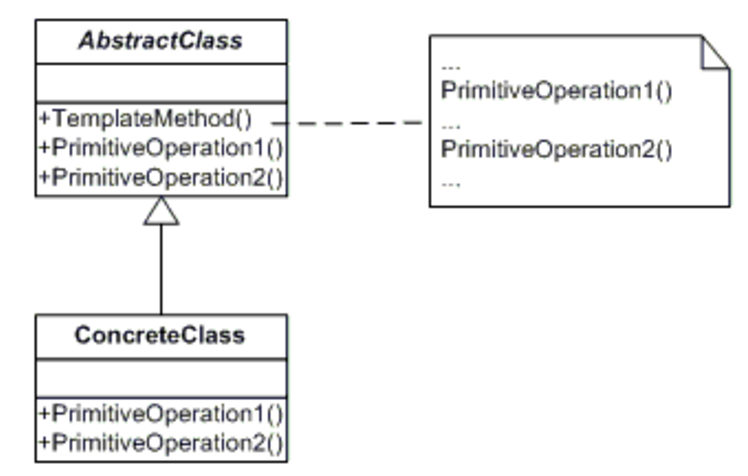
\includegraphics[scale=0.75]{pics/template.png}

\end{itemize}




\ifx \allfiles \undefined
%\end{CJK*}
\end{document}
\fi
